\documentclass{article}

% if you need to pass options to natbib, use, e.g.:
%     \PassOptionsToPackage{numbers, compress}{natbib}
% before loading neurips_2024


% ready for submission
% \usepackage{neurips_2024}


% to compile a preprint version, e.g., for submission to arXiv, add add the
% [preprint] option:
% \usepackage[preprint]{neurips_2024}


% to compile a camera-ready version, add the [final] option, e.g.:
    \usepackage[final]{neurips_2024}


% to avoid loading the natbib package, add option nonatbib:
%    \usepackage[nonatbib]{neurips_2024}
% \usepackage{natbib}
% \usepackage[numbers]{natbib}
% \usepackage{cite}
% \usepackage{citep}
\usepackage[utf8]{inputenc} % allow utf-8 input
\usepackage[T1]{fontenc}    % use 8-bit T1 fonts
\usepackage{hyperref}       % hyperlinks
\usepackage{url}            % simple URL typesetting
\usepackage{booktabs}       % professional-quality tables
\usepackage{amsfonts}       % blackboard math symbols
\usepackage{nicefrac}       % compact symbols for 1/2, etc.
\usepackage{microtype}      % microtypography
\usepackage{xcolor}         % colors
\usepackage{graphicx}
\usepackage{times}
\usepackage{latexsym}
\usepackage{amssymb}
\usepackage{hyperref}
\usepackage{url}
\usepackage{booktabs}
\usepackage{color}
\usepackage{xcolor}
% \usepackage{fancyvrb}
\usepackage{markdown}
% \usepackage{minted}
% \usepackage{listings}
% \lstset{breaklines=true}
% \usepackage{tcolorbox}
\usepackage[most]{tcolorbox}
\usepackage{multirow} % 用于合并多行
\usepackage{tabularx} % 用于自动换行
\usepackage{booktabs} % 用于绘制漂亮的表格边框
\usepackage{array}    % 用于调整列宽
\usepackage{longtable}  % 引入longtable包
\usepackage{pgfplots}
\usepackage{float}
\usepackage{IEEEtrantools}
\usepackage{amsmath}
\usepackage{titlesec}

\usetikzlibrary{patterns}

\newcommand{\lmxue}[1]{\textcolor{blue}{Liumeng: {#1}}}
\newcommand{\comments}[1]{\textcolor{red}{Comments: {#1}}}
\newcommand{\ziya}[1]{\textcolor{blue}{Ziya: {#1}}}
\def\xue#1{{\color{cyan}{\bf [Xue:} {{#1}}{\bf ]}}}



\title{Audio-FLAN: A Preliminary Release}

% The \author macro works with any number of authors. There are two commands
% used to separate the names and addresses of multiple authors: \And and \AND.
%
% Using \And between authors leaves it to LaTeX to determine where to break the
% lines. Using \AND forces a line break at that point. So, if LaTeX puts 3 of 4
% authors names on the first line, and the last on the second line, try using
% \AND instead of \And before the third author name.

\author{
    \IEEEauthorblockN{Liumeng Xue$^{a,b*}$, Ziya Zhou$^{a,b*}$, Jiahao Pan$^{a,b}$}
    \IEEEauthorblockN{\textbf{Zixuan Li$^{c}$, Shuai Fan$^{d}$, Yinghao Ma$^{e,b}$, Sitong Cheng$^{a}$}}
    \IEEEauthorblockN{\textbf{Dongchao Yang$^{f}$, Haohan Guo$^{f}$, Yujia Xiao$^{f}$, Xinsheng Wang$^{a}$}}
    \IEEEauthorblockN{\textbf{Zixuan Shen$^{a}$, Chuanbo Zhu$^{a}$, Xinshen Zhang$^{a}$, Tianchi Liu{$^g$}}}
    \IEEEauthorblockN{\textbf{Ruibin Yuan$^{a,b}$, Zeyue Tian$^{a,b}$, Haohe Liu$^{b,h}$, Emmanouil Benetos$^{b,e}$, Ge Zhang$^{b}$}}
    \IEEEauthorblockN{\textbf{Yike Guo$^{a}$, Wei Xue$^{a}$}}
    \vspace{0.1in}
    \IEEEauthorblockA{$^a$ The Hong Kong University of Science and Technology, $^b$ M-A-P}
    % \IEEEauthorblockA{$^b$ M-A-P}\\
    \IEEEauthorblockA{$^c$ Inner Mongolia University, $^d$ Beihang University}
    % \IEEEauthorblockA{$^d$ Beihang University}\\
    \IEEEauthorblockA{$^e$ Queen Mary University of London, $^f$ The Chinese University of Hong Kong}
    % \IEEEauthorblockA{$^f$ The Chinese University of Hong Kong}\\
    \IEEEauthorblockA{$^g$ National University of Singapore, $^h$ University of Surrey}
    % \IEEEauthorblockA{$^h$ University of Surrey}\\
    % \IEEEauthorblockA{\{lmxue, yikeguo, weixue\}@ust.hk, zzhoucp@connect.ust.hk}
}


% \linespread{1.2}


% \usepackage[a4paper, top=1.5in, bottom=1.5in, left=1in, right=1in]{geometry}  % 自定义页边距

% 重新定义文本区域宽度和高度,扩大正文区域
\AtBeginDocument{
  \newgeometry{
    textheight=9in,    % 正文高度
    textwidth=6.5in,   % 正文宽度,扩大为6.5英寸
    top=1.5in,         % 顶部边距
    bottom=1.5in,      % 底部边距
    left=1in,          % 左边距
    right=1in,         % 右边距
    headheight=12pt,   % 页眉高度
    headsep=25pt,      % 页眉与正文的距离
    footskip=30pt      % 页脚与正文的距离
  }
}
\begin{document}

\maketitle
\begin{abstract}

Hierarchical clustering is a powerful tool for exploratory data analysis, organizing data into a tree of clusterings from which a partition can be chosen. This paper generalizes these ideas by proving that, for any reasonable hierarchy, one can optimally solve any center-based clustering objective over it (such as $k$-means). Moreover, these solutions can be found exceedingly quickly and are \emph{themselves} necessarily hierarchical. 
%Thus, given a cluster tree, we show that one can quickly generate a myriad of \emph{new} hierarchies from it. 
Thus, given a cluster tree, we show that one can quickly access a plethora of new, equally meaningful hierarchies.
Just as in standard hierarchical clustering, one can then choose any desired partition from these new hierarchies. We conclude by verifying the utility of our proposed techniques across datasets, hierarchies, and partitioning schemes.


\end{abstract}

\section{Introduction}

% Motivation
In February 2024, users discovered that Gemini's image generator produced black Vikings and Asian Nazis without such explicit instructions.
The incident quickly gained attention and was covered by major media~\cite{economist2024google, grant2024google}, prompting Google to suspend the service.
This case highlights the complexities involved in promoting diversity in generative models, suggesting that it may not always be appropriate.
Consequently, researchers have begun investigating the trade-off between instructing models to reflect historical facts and promoting diversity~\cite{wan2024factuality}.
Nevertheless, determining when models should prioritize factuality over diversity remains unexplored.

\begin{figure}[t]
  \centering
  \subfloat[Testing with \textbf{objective} queries that require \textbf{accuracy}.]{
    \includegraphics[width=1.0\linewidth]{Figures/obj-cover.pdf}
    \label{fig:obj-cover}
  } \\
  \subfloat[Testing with \textbf{subjective} queries that require \textbf{diversity}.]{
    \includegraphics[width=1.0\linewidth]{Figures/subj-cover.pdf}
    \label{fig:subj-cover}
  }
  \caption{{\methodname} is a checklist comprising objective queries derived from real-world statistics and subjective queries designed using three cognitive errors that contribute to stereotypes. It includes queries designed for LLMs and T2I models.}
\end{figure}

% Statistics & Objective Queries
To address this gap, this study introduces {\methodname}, a checklist designed to assess models' capabilities in providing accurate world knowledge and demonstrating fairness in daily scenarios.
For world knowledge assessment, we collect 19 key statistics on U.S. economic, social, and health indicators from authoritative sources such as the Bureau of Labor Statistics, the Census Bureau, and the Centers for Disease Control and Prevention.
Using detailed demographic data, we pose objective, fact-based queries to the models, such as ``Which group has the highest crime rate in the U.S.?''—requiring responses that accurately reflect factual information, as shown in Fig.~\ref{fig:obj-cover}.
Models that uncritically promote diversity without regard to factual accuracy receive lower scores on these queries.

% Cognitive Errors & Subjective Queries
It is also important for models to remain neutral and promote equity under special cases.
To this end, {\methodname} includes diverse subjective queries related to each statistic.
Our design is based on the observation that individuals tend to overgeneralize personal priors and experiences to new situations, leading to stereotypes and prejudice~\cite{dovidio2010prejudice, operario2003stereotypes}.
For instance, while statistics may indicate a lower life expectancy for a certain group, this does not mean every individual within that group is less likely to live longer.
Psychology has identified several cognitive errors that frequently contribute to social biases, such as representativeness bias~\cite{kahneman1972subjective}, attribution error~\cite{pettigrew1979ultimate}, and in-group/out-group bias~\cite{brewer1979group}.
Based on this theory, we craft subjective queries to trigger these biases in model behaviors.
Fig.~\ref{fig:subj-cover} shows two examples on AI models.

% Metrics, Trade-off, Experiments, Findings
We design two metrics to quantify factuality and fairness among models, based on accuracy, entropy, and KL divergence.
Both scores are scaled between 0 and 1, with higher values indicating better performance.
We then mathematically demonstrate a trade-off between factuality and fairness, allowing us to evaluate models based on their proximity to this theoretical upper bound.
Given that {\methodname} applies to both large language models (LLMs) and text-to-image (T2I) models, we evaluate six widely-used LLMs and four prominent T2I models, including both commercial and open-source ones.
Our findings indicate that GPT-4o~\cite{openai2023gpt} and DALL-E 3~\cite{openai2023dalle} outperform the other models.
Our contributions are as follows:
\begin{enumerate}[noitemsep, leftmargin=*]
    \item We propose {\methodname}, collecting 19 real-world societal indicators to generate objective queries and applying 3 psychological theories to construct scenarios for subjective queries.
    \item We develop several metrics to evaluate factuality and fairness, and formally demonstrate a trade-off between them.
    \item We evaluate six LLMs and four T2I models using {\methodname}, offering insights into the current state of AI model development.
\end{enumerate}
% 
\section{Related Work}

\subsection{Instruction Generation}

Instruction tuning is essential for aligning Large Language Models (LLMs) with user intentions~\cite{ouyang2022training,cao2023instruction}. Initially, this involved collecting and cleaning existing data, such as open-source NLP datasets~\cite{wang2023far,ding2023enhancing}. With the importance of instruction quality recognized, manual annotation methods emerged~\cite{wang2023far,zhou2024lima}. As larger datasets became necessary, approaches like Self-Instruct~\cite{wang2022self} used models to generate high-quality instructions~\cite{guo2024human}. However, complex instructions are rare, leading to strategies for synthesizing them by extending simpler ones~\cite{xu2023wizardlm,sun2024conifer,he2024can}. However, existing methods struggle with scalability and diversity.


\subsection{Back Translation}

Back-translation, a process of translating text from the target language back into the source language, is mainly used for data augmentation in tasks like machine translation~\cite{sennrich2015improving, hoang2018iterative}. ~\citet{li2023self} first applied this to large-scale instruction generation using unlabeled data, with Suri~\cite{pham2024suri} and Kun~\cite{zheng2024kun} extending it to long-form and Chinese instructions, respectively. ~\citet{nguyen2024better} enhanced this method by adding quality assessment to filter and revise data. Building on this, we further investigated methods to generate high-quality complex instruction dataset using back-translation.


\begin{figure*}[ht]
    \centering
    \includegraphics[width=\textwidth, trim=79 280 93 123, clip]{figures/framework_img.pdf}
    \caption{The pipeline of the \ENDow{} framework 
    %where each component is specified in a given configuration. 
    which yields a downstream task score and a WER score of the transcript set input to the task. The pipeline is executed for several severeties of noising and types of cleaning techniques. %Acoustic noising is applied at $k$ intensities, providing $k+1$ audio versions (including the non-noised version), eventually producing $k+2$ transcript versions (including the source transcript). Applying transcript cleaning reveals the effect of \textit{types} of noise. 
    Resulting scores are plotted on a graph for the analyses, as in, e.g., \autoref{fig_cleaning_graphs}.}
    %The pipeline is executed on $k+1$ intensities of acoustic noising (including the non-noised version), producing $k+2$ scores for the downstream task (including execution on the source transcripts). This process eventually describes the effect of the \textit{intensity} of transcript noise on the downstream task. The process is repeated for $m$ cleaning techniques ($m+1$ when including no cleaning), to analyze the benefit of a cleaning approach and the effect of the \textit{types} of transcript noise.}
    \label{fig_framework}
\end{figure*}

\section{Methodology}
This section presents our neural approach to preconditioning PDEs. We begin by formulating the problem and discretizing the governing PDEs in Section~\ref{subsec:problem_formulation}, followed by an overview of the Neural Preconditioning Operator (NPO) framework in Section~\ref{subsec:npo_framework}. Next, we define the learning objectives for training the NPO in Section~\ref{subsec:learning_npo}, and conclude with a detailed description of the Neural Algebraic Multigrid (NAMG) Operator in Section~\ref{subsec:npo_amg}, which combines classical multigrid principles with neural attention for efficient coarse-grid correction.

\subsection{Problem Formulation}
\label{subsec:problem_formulation}
We consider PDEs on a domain \(D \subset \mathbb{R}^d\), with functions from the input and solution spaces \(\mathcal{A}(D; \mathbb{R}^{d_a})\) and \(\mathcal{U}(D; \mathbb{R}^{d_u})\), respectively. The operator \(\mathcal{G}: \mathcal{A} \to \mathcal{U}\) is expressed as an integral:
\begin{equation}
    \mathcal{G}a(\mathbf{x}) = \int_{D} \kappa(\mathbf{x}, \mathbf{y}) \, a(\mathbf{y}) \, d\mathbf{y},
\end{equation}
where \(\kappa: D \times D \to \mathbb{R}\) is the kernel function.

After discretization, the PDE leads to a sparse, symmetric positive definite (SPD) matrix \(A \in \mathbb{R}^{n \times n}\) and a right-hand side vector \(\mathbf{f} \in \mathbb{R}^n\). Our goal is to learn a preconditioner \(M = \mathcal{M}_{\theta}(A, \mathbf{f})\), defined by:
\begin{equation}
    M \;=\; \mathcal{M}_{\theta}(A),
\end{equation}

where \(\theta\) are the learned parameters. The preconditioner \(M\) is trained to remain SPD and efficient to apply, improving the condition number of \(A\) and accelerating iterative solvers.

\subsection{Neural Preconditioning Operator Framework}
\label{subsec:npo_framework}
Figure~\ref{fig:framework} illustrates the two-phase workflow of our Neural Preconditioning Operator (NPO) framework, consisting of \emph{training} (Figure~\ref{fig:framework}(a)) and \emph{solving} (Figure~\ref{fig:framework}(b)). 

During the training phase, the NPO takes the system matrix \(A\) and right-hand side vector \(f\) as inputs and generates an intermediate output, including a preconditioner matrix \(M\), the solution approximation \(u\), and residual \(r\). Three loss functions are used to guide the optimization: the \emph{data loss} (from \(u\) and \(f\)), \emph{residual loss} (from \(r\)), and \emph{condition loss} (from \(M\)). The NPO's parameters \(\theta\) are updated by minimizing the sum of these losses.

Once trained, the NPO is applied in the solving phase to accelerate iterative Krylov subspace methods (e.g., CG or GMRES). Given a new system \(A\mathbf{x} = \mathbf{b}\), the solver repeatedly uses the learned \(M\) to compute preconditioned residuals \(z = M r\), significantly reducing iteration counts and improving convergence efficiency across various PDE systems and mesh types.

\subsection{Learning Neural Preconditioner Operator}
\label{subsec:learning_npo}
To train a neural preconditioner \( \mathcal{M}_{\theta}(A) \), we define two complementary loss functions: a \emph{condition loss} and a \emph{residual loss}. These losses guide the preconditioner to behave like \( A^{-1} \), improving both the spectral properties of the system and solution accuracy.

\subsubsection{Condition Loss}

A preconditioner that approximates \( A^{-1} \) should ensure that \( A \mathcal{M}_{\theta}(A) \approx I \). A natural objective is to minimize:
\begin{equation}
    \label{eq:inverse_loss}
    \bigl\| I - A\,\mathcal{M}_{\theta}(A) \bigr\|_F^2.
\end{equation}
However, directly optimizing this matrix norm is computationally infeasible for large systems. Instead, we define a condition loss over sampled residuals \(\mathbf{r}_i\) to achieve a similar effect:
\begin{equation}
    \label{eq:condition_loss}
    \min_{\theta} \frac{1}{N} \sum_{i=1}^{N} \bigl\| \bigl(I - A_i\,\mathcal{M}_{\theta}(A_i)\bigr)\,\mathbf{r}_i \bigr\|_2^2.
\end{equation}

This condition loss indirectly improves the system's spectral properties, reducing the condition number of the preconditioned matrix and thereby accelerating convergence in iterative solvers.

\subsubsection{Residual Loss}

While the condition loss ensures better spectral properties, it does not directly assess how well the preconditioner solves the system for the right-hand side \(\mathbf{b}_i\). To address this, we define a residual loss that measures the accuracy of the preconditioner when applied to \(\mathbf{b}_i\):
\begin{equation}
    \label{eq:residual_loss}
    \min_{\theta \in \Theta} 
    \frac{1}{N}
    \sum_{i=1}^{N}
    \bigl\|
       A_{i}\mathcal{M}_{\theta}(A_i)\bigl(\mathbf{b}_i\bigr)
       \;-\;
       \mathbf{b}_i
    \bigr\|_2^2.
\end{equation}

This loss encourages \( \mathcal{M}_{\theta}(A) \) to approximate \( A^{-1} \) by minimizing the discrepancy between the predicted and actual right-hand side. Together, the condition and residual losses promote a preconditioner that reduces both spectral issues and iteration counts, enabling faster and more robust convergence for a wide range of PDE systems.

\subsection{Neural Algebraic Multigrid Operator}
\label{subsec:npo_amg}

The Neural Algebraic Multigrid (NAMG) Operator enhances the classical AMG framework by introducing neural attention mechanisms for efficient feature aggregation and prolongation. The process involves three main steps: restriction, attention-based coarse-grid correction, and prolongation.

\subsubsection{Restriction and Coarse Feature Aggregation}

Given fine-grid features \( \mathbf{x}^{f} \in \mathbb{R}^{N \times C} \) and the adjacency matrix \( A \in \mathbb{R}^{N \times N} \), restriction is defined as:

\begin{equation}
    \mathbf{x}^{c} = R \mathbf{x}^{f}, \quad R = A \cdot E_{\theta},
\end{equation}

where \( E_{\theta} \) contains learned attention weights:

\begin{equation}
    e_{ji} = \frac{\exp(\mathbf{W}_{\text{coarse}} \mathbf{x}_{i}^{f} / \tau)}{\sum_{i' \in \mathcal{N}_j} A_{ji'} \exp(\mathbf{W}_{\text{coarse}} \mathbf{x}_{i'}^{f} / \tau)}.
\end{equation}

Here, \( \mathcal{N}_j \) denotes the neighbors of node \( j \), \( \mathbf{W}_{\text{coarse}} \) is a learnable weight matrix, and \( \tau \) is a scaling parameter. Coarse features are computed by aggregating fine-grid tokens using these weights.

\subsubsection{Attention-Based Coarse Correction}

The coarse-grid features are refined through self-attention. Queries, keys, and values are computed as:

\begin{equation}
    \mathbf{q} = \mathbf{W}_{q} \mathbf{x}^{c}, \quad \mathbf{k} = \mathbf{W}_{k} \mathbf{x}^{c}, \quad \mathbf{v} = \mathbf{W}_{v} \mathbf{x}^{c}.
\end{equation}

Attention scores are then used to update the coarse features:

\begin{equation}
    \mathbf{x}_{j}^{c, \text{updated}} = \sum_{k} \text{softmax}\left( \frac{\mathbf{q}_{j} \cdot \mathbf{k}_{k}^{\top}}{\sqrt{C}} \right) \mathbf{v}_{k}.
\end{equation}

\subsubsection{Prolongation and Fine-Grid Correction}

The updated coarse features are projected back to the fine grid:

\begin{equation}
    \mathbf{x}'^{f} = \mathbf{x}^{f} + P \mathbf{x}'^{c}, \quad P = A \cdot E_{\theta}^{\top}.
\end{equation}

This process dynamically adjusts restriction and prolongation through learned attention, allowing the operator to capture complex patterns inherent in PDEs across diverse domains. 


\begin{figure*}[t]
    \centering
    \small
    \hspace*{-1.2cm}
    \subfigure[Alignment stage]{
    \begin{minipage}[t]{0.24\linewidth}
    \centering
      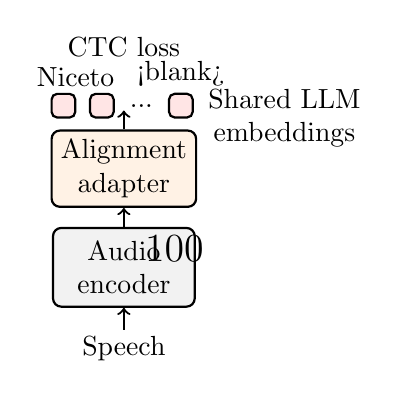
\begin{tikzpicture} [scale=0.8]
        \node(ae) at (0,0) [rectangle, draw=black, fill=gray!10, rounded corners=3pt, thick, minimum width=1.8cm,minimum height=1cm,align=center] {Audio\\encoder};
        \node(freeze) at ([xshift=0.8cm,yshift=0.3cm]ae.center) [rectangle, align=center] {\Large{\ding{100}}};
        \node(fb) at ([yshift=-0.3cm]ae.south) [rectangle, align=center,anchor=north] {Speech};
        \node(aa) at ([yshift=0.3cm]ae.north) [rectangle, draw=black, fill=orange!10, rounded corners=3pt, thick, minimum width=1.8cm,minimum height=0.5cm,align=center,anchor=south] {Alignment\\adapter};
        
        \node(f1) at ([yshift=1.0cm]aa.west) [rectangle, draw=black, fill=red!10, rounded corners=2pt, thick, minimum width=0.3cm, minimum height=0.3cm,align=center,anchor=west] {};
        \node(f2) at ([xshift=0.2cm]f1.east) [rectangle, draw=black, fill=red!10, rounded corners=2pt, thick, minimum width=0.3cm, minimum height=0.3cm,align=center,anchor=west] {};
        \node(f3) at ([xshift=0.075cm]f2.east) [rectangle, draw=white,  thick, align=center,anchor=west] {...};
        \node(f4) at ([xshift=0.075cm]f3.east) [rectangle, draw=black, fill=red!10, rounded corners=2pt, thick, minimum width=0.3cm, minimum height=0.3cm,align=center,anchor=west] {};
        \node(t1) at ([yshift=-0.05cm]f1.north) [rectangle, align=center,anchor=south] {Nice};
        \node(t2) at ([yshift=-0.05cm]f2.north) [rectangle, align=center,anchor=south] {to};
        \node(t4) at ([yshift=-0.05cm]f4.north) [rectangle, align=center,anchor=south] {<blank>};
        \node(se) at ([xshift=0.075cm,yshift=-0.2cm]f4.east) [rectangle, align=center,anchor=west] {Shared LLM\\embeddings};
        \node(ctc) at ([yshift=1.0cm]aa.north) [rectangle, rounded corners=3pt, thick, align=center,anchor=south] {CTC loss};

        
        \draw[->,thick]([yshift=-0.05cm]fb.north)--(ae.south);
        \draw[->,thick](ae.north)--(aa.south);
        \draw[->,thick](aa.north)--([yshift=0.3cm]aa.north);

        
      \end{tikzpicture}
    \end{minipage}
    }
    \subfigure[Shrinking stage]{
    \begin{minipage}[t]{0.45\linewidth}
    \centering
    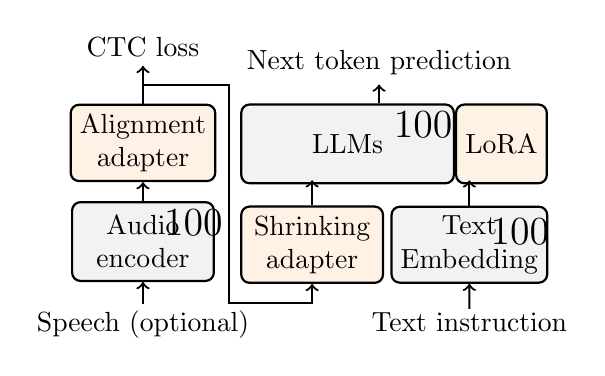
\begin{tikzpicture} [scale=0.8]
        \node(ae) at (0,0) [rectangle, draw=black, fill=gray!10, rounded corners=3pt, thick, minimum width=1.8cm,minimum height=1cm,align=center] {Audio\\encoder};
        \node(freeze) at ([xshift=0.8cm,yshift=0.3cm]ae.center) [rectangle, align=center] {\Large{\ding{100}}};
        \node(fb) at ([yshift=-0.3cm]ae.south) [rectangle, align=center,anchor=north] {Speech (optional)};
        \node(aa) at ([yshift=0.3cm]ae.north) [rectangle, draw=black, fill=orange!10, rounded corners=3pt, thick, minimum width=1.8cm,minimum height=0.5cm,align=center,anchor=south] {Alignment\\adapter};
        \node(ctc) at ([yshift=0.6cm]aa.north) [rectangle,align=center,anchor=south] {CTC loss};
        \node(sa) at ([xshift=0.4cm,yshift=-0.05cm]ae.east) [rectangle, draw=black, fill=orange!10, rounded corners=3pt, thick, minimum width=1.8cm,minimum height=0.5cm,align=center,anchor=west] {Shrinking\\adapter};
        \node(llm) at ([yshift=1.6cm]sa.west) [rectangle, draw=black, fill=gray!10, rounded corners=3pt, thick, minimum width=2.7cm,minimum height=1.0cm,align=center,anchor=west] {LLMs};
        \node(lora) at (llm.east) [rectangle, draw=black, fill=orange!10, rounded corners=3pt, thick, minimum width=1.0cm,minimum height=1.0cm,align=center,anchor=west] {LoRA};
        \node(te) at ([xshift=0.1cm]sa.east) [rectangle, draw=black, fill=gray!10, rounded corners=3pt, thick, minimum width=1.8cm,minimum height=0.5cm,align=center,anchor=west] {Text\\Embedding};
        \node(freeze3) at ([xshift=0.8cm,yshift=0.2cm]te.center) [rectangle, align=center] {\Large{\ding{100}}};
        \node(ti) at ([yshift=-0.3cm]te.south) [rectangle, align=center,anchor=north] {Text instruction};
        \node(freeze2) at ([xshift=1.2cm,yshift=0.3cm]llm.center) [rectangle, align=center] {\Large{\ding{100}}};
        \node(loss) at ([xshift=0.5cm, yshift=0.3cm]llm.north) [rectangle, align=center,anchor=south] {Next token prediction};

        
        \draw[->,thick]([yshift=-0.05cm]fb.north)--(ae.south);
        \draw[->,thick](ae.north)--(aa.south);
        \draw[->,thick](aa.north)--(ctc.south);
        \draw[->,thick](sa.north)--([yshift=0.4cm]sa.north);
        \draw[->,thick](te.north)--([yshift=0.4cm]te.north);
        \draw[->,thick]([yshift=-0.3cm]loss.south)--(loss.south);
        \draw[->,thick]([yshift=-0.1cm]ti.north)--(te.south);

        \draw[->,thick](aa.north)--([yshift=0.3cm]aa.north)--([xshift=0.2cm, yshift=0.3cm]aa.north -| aa.east)--([xshift=0.2cm, yshift=-0.3cm]sa.south -| aa.east)--([yshift=-0.3cm]sa.south)--(sa.south);
      \end{tikzpicture}
    \end{minipage}
    }
    \subfigure[SFT stage]{
    \begin{minipage}[t]{0.20\linewidth}
    \centering
    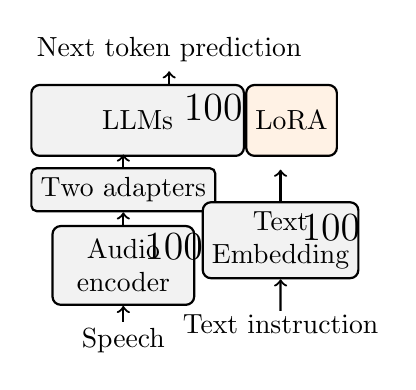
\begin{tikzpicture} [scale=0.8]
        \node(ae) at (0,0) [rectangle, draw=black, fill=gray!10, rounded corners=3pt, thick, minimum width=1.8cm,minimum height=1cm,align=center] {Audio\\encoder};
        \node(freeze) at ([xshift=0.8cm,yshift=0.3cm]ae.center) [rectangle, align=center] {\Large{\ding{100}}};
        \node(fb) at ([yshift=-0.2cm]ae.south) [rectangle, align=center,anchor=north] {Speech};
        \node(aa) at ([yshift=0.2cm]ae.north) [rectangle, draw=black, fill=gray!10, rounded corners=2pt, thick, minimum width=1.8cm,minimum height=0.5cm,align=center,anchor=south] {Two adapters};
        
        \node(llm) at ([yshift=1.1cm]aa.west) [rectangle, draw=black, fill=gray!10, rounded corners=3pt, thick, minimum width=2.7cm,minimum height=0.9cm,align=center,anchor=west] {LLMs};
        \node(lora) at (llm.east) [rectangle, draw=black, fill=orange!10, rounded corners=3pt, thick, minimum width=0.9cm,minimum height=0.9cm,align=center,anchor=west] {LoRA};
        \node(te) at ([xshift=0.1cm,yshift=0.4cm]ae.east) [rectangle, draw=black, fill=gray!10, rounded corners=3pt, thick, minimum width=1.8cm,minimum height=0.5cm,align=center,anchor=west] {Text\\Embedding};
        \node(freeze3) at ([xshift=0.8cm,yshift=0.2cm]te.center) [rectangle, align=center] {\Large{\ding{100}}};
        \node(ti) at ([yshift=-0.4cm]te.south) [rectangle, align=center,anchor=north] {Text instruction};
        \node(freeze2) at ([xshift=1.2cm,yshift=0.2cm]llm.center) [rectangle, align=center] {\Large{\ding{100}}};
        \node(loss) at ([xshift=0.5cm, yshift=0.2cm]llm.north) [rectangle, align=center,anchor=south] {Next token prediction};
       
        \draw[->,thick]([yshift=-0.05cm]fb.north)--(ae.south);
        \draw[->,thick](ae.north)--(aa.south);
        \draw[->,thick](aa.north)--([yshift=0.2cm]aa.north);
        \draw[->,thick](te.north)--([yshift=0.5cm]te.north);
        \draw[->,thick]([yshift=-0.2cm]loss.south)--(loss.south);
        \draw[->,thick]([yshift=-0.1cm]ti.north)--(te.south);
        
      \end{tikzpicture}
    \end{minipage}
    }
      \caption{Training progress of Soundwave. The gray modules are frozen while the orange modules are updated.}
      \label{architecture}
  \end{figure*}

  



\section{Fine-Tuning Experiments}
This section validates that our dataset can enhance the GUI grounding capabilities of VLMs and that the proposed functionality grounding and referring are effective fine-tuning tasks.
\subsection{Experimental Settings}
\noindent\textbf{Evaluation Benchmarks} We base our evaluation on the UI grounding benchmarks for various scenarios: \textbf{FuncPred} is the test split from our collected functionality dataset. This benchmark requires a model to locate the element specified by its functionality description. \textbf{ScreenSpot}~\citep{cheng2024seeclick} is a benchmark comprising test samples on mobile, desktop, and web platforms. It requires the model to locate elements based on short instructions. \textbf{RefExp}~\citep{Bai2021UIBertLG} is to locate elements given crowd-sourced referring expressions. \textbf{VisualWebBench (VWB)}~\citep{liu2024visualwebbench} is a comprehensive multi-modal benchmark assessing the understanding capabilities of VLMs in web scenarios. We select the element and action grounding tasks from this benchmark. To better align with high-level semantic instructions for potential agent requirements and avoid redundancy evaluation with ScreenSpot, we use ChatGPT to expand the OCR text descriptions in the original task instructions, such as \textit{Abu Garcia College Fishing} into functionality descriptions like \textit{This element is used to register for the Abu Garcia College Fishing event}.
\textbf{MOTIF}~\citep{Burns2022ADF} requires an agent to complete a natural language command in mobile Apps.
For all of these benchmarks, we report the grounding accuracy (\%): $\text { Acc }= \sum_{i=1}^N \mathbf{1}\left(\text {pred}_i \text { inside GT } \text {bbox}_i\right) / N \times 100 $ where $\mathbf{1}$ is an indicator function and $N$ is the number of test samples. This formula denotes the percentage of samples with the predicted points lying within the bounding boxes of the target elements.

\noindent\textbf{Training Details}
We select Qwen-VL-10B~\citep{bai2023qwen} and SliME-8B~\citep{slime} as the base models and fine-tune them on 25k, 125k, and 702k samples of the AutoGUI training data to investigate how the AutoGUI data enhances the UI grounding capabilities of the VLMs. The models are fine-tuned on 8 A100 GPUs for one epoch. We follow SeeClick~\citep{cheng2024seeclick} to fine-tune Qwen-VL with LoRA~\citep{hu2022lora} and follow the recipe of SliME~\citep{slime} to fine-tune it with only the visual encoder frozen (More details in Sec.~\ref{sec:supp:impl details}).

\noindent\textbf{Compared VLMs}
We compare with both general-purpose VLMs (i.e., LLaVA series~\citep{liu2023llava,liu2024llavanext}, SliME~\citep{slime}, and Qwen-VL~\citep{bai2023qwen}) and UI-oriented ones (i.e., Qwen2-VL~\citep{qwen2vl}, SeeClick~\citep{cheng2024seeclick}, CogAgent~\citep{hong2023cogagent}). SeeClick finetunes Qwen-VL with around 1 million data combining various data sources, including a large proportion of human-annotated UI grounding/referring samples. CogAgent is trained with a huge amount of text recognition, visual grounding, UI understanding, and publicly available text-image datasets, such as LAION-2B~\citep{LAION5B}. During the evaluation, we manually craft grounding prompts suitable for these VLMs.
\subsection{Experimental Results and Analysis}
\begin{table}[]
\scriptsize
\centering
\caption{\textbf{Element grounding accuracy on the used benchmarks.} We compare the base models fine-tuned with our AutoGUI data and representative open-source VLMs. The results show that the two base models (i.e. Qwen-VL and SliME-8B) obtain significant performance gains over the benchmarks after being fine-tuned with AutoGUI data. Moreover, increasing the AutoGUI data size consistently improves grounding accuracy, demonstrating notable scaling effects. $\dag$ means the metric value is borrowed from the benchmark paper. $*$ means using additional SeeClick training data.}
\label{tab:eval results}
\begin{tabular}{@{}cccccccccc@{}}
\toprule
Type & Model    & Size    & FuncPred & VWB EG & VWB AG & MoTIF & RefExp & ScreenSpot  \\ \midrule
\multirow{5}{*}{General} & LLaVA-1.5~\citep{liu2023llava} & 7B & 3.2      &        12.1$^{\dag}$        &     13.6$^{\dag}$           &  7.2   &  4.2 & 5.0 & \\
 & LLaVA-1.5~\citep{liu2023llava} & 13B & 5.8      &           16.7     &        9.7        &   12.3 &  20.3   & 11.2 &  \\
 & LLaVA-1.6~\citep{liu2024llavanext} & 34B &  4.4      &      19.9          &    17.0            &   7.0 &  29.1  & 10.3 &  \\
 & SliME~\citep{slime} & 8B &  3.2  &   6.1       &     4.9     & 7.0  &  8.3  &  13.0  \\ 

 & Qwen-VL~\citep{bai2023qwen} & 10B &  3.0     &      1.7          &      3.9          &    7.8 &  8.0  & 5.2$^{\dag}$   \\ 
 \midrule
\multirow{3}{*}{UI-VLM} &  Qwen2-VL~\citep{bai2023qwen}  & 7B     &     7.8       &    3.9        &  3.9  &  16.7 & 32.4 & 26.1    \\
 & CogAgent~\citep{hong2023cogagent} & 18B    &  29.3   &    \underline{55.7}      &    \textbf{59.2}      & \textbf{24.7}   & 35.0 &  47.4$^{\dag}$  \\
 & SeeClick~\citep{cheng2024seeclick} & 10B    &    19.8     &    39.2           &     27.2           & 11.1  &  \textbf{58.1}  & \underline{53.4}$^{\dag}$ \\ 
\midrule
\multirow{4}{*}{Finetuned} &  Qwen-VL-AutoGUI25k & 10B      &    14.2     &      12.8         &    12.6           &   10.8    &  12.0 & 19.0    \\
 & Qwen-VL-AutoGUI125k  & 10B       &     25.5     &      23.2         &        29.1       &    11.5   &  14.9 & 32.0     \\ 
 & Qwen-VL-AutoGUI702k  & 10B       &   43.1   &    38.0       &     32.0    &  15.5  & 23.9 &    38.4   \\
& Qwen-VL-AutoGUI702k$^*$   & 10B     &  \underline{50.0}  &    \textbf{56.2}    &  \underline{45.6}  & \underline{21.0} & \underline{51.5} & \textbf{54.2}      \\
\midrule
\multirow{3}{*}{Finetuned} & SliME-AutoGUI25k  & 8B     &   28.0   &     14.0      &      10.6      &  14.3   & 18.4 & 27.2   \\
 & SliME-AutoGUI125k   & 8B      &   39.9    &  22.0   &     12.0       &  17.8  & 22.1 &  35.0     \\
 & SliME-AutoGUI702k   & 8B      &     \textbf{62.6}   &       25.4        &     13.6          &   20.6    & 26.7 & 44.0 &          \\
\bottomrule
\end{tabular}
\end{table}
\vspace{-2mm}


\noindent\textbf{A) AutoGUI functionality annotations effectively enhance VLMs' UI grounding capabilities and achieve scaling effects.} We endeavor to show that the element functionality data autonomously collected by AutoGUI contributes to high grounding accuracy. The results in Tab.~\ref{tab:eval results} demonstrate that on all benchmarks the two base models achieve progressively rising grounding accuracy as the functionality data size scales from 25k to 702k, with SliME-8B's accuracy increasing from merely \textbf{3.2} and \textbf{13.0} to \textbf{62.6} and \textbf{44.0} on FuncPred and ScreenSpot, respectively. This increase is visualized in Fig.~\ref{fig:funcpred scaling success} showing that increasing AutoGUI data amount leads to more precise localization performance.

After fine-tuning with AutoGUI 702k data, the two base models surpass SeeClick, the strong UI-oriented VLM on FuncPred and MOTIF. We notice that the base models lag behind SeeClick and CogAgent on ScreenSpot and RefExp, as the two benchmarks contain test samples whose UIs cannot be easily recorded (e.g., Apple devices and Desktop software) as training data, causing a domain gap. Nevertheless, SliME-8B still exhibits noticeable performance improvements on ScreenSpot and RefExp when scaling up the AutoGUI data, suggesting that the AutoGUI data helps to enhance grounding accuracy on the out-of-domain tasks.

To further unleash the potential of the AutoGUI data, the base model, Qwen-VL, is finetuned with the combination of the AutoGUI and SeeClick UI-grounding data. This model becomes the new state-of-the-art on FuncPred, ScreenSpot, and VWB EG, surpassing SeeClick and CogAgent. This result suggests that our AutoGUI data can be mixed with existing UI grounding training data to foster better UI grounding capabilities.

In summary, our functionality data can endow a general VLM with stronger UI grounding ability and exhibit clear scaling effects as the data size increases.


\begin{table}[]
\centering
\footnotesize
\caption{\textbf{Comparing the AutoGUI functionality annotation type with existing types}. Qwen-VL is fine-tuned with the three annotation types. The results show that our functionality data leads to superior grounding accuracy compared with the naive element-HTML data and the condensed functionality annotations.}
\label{tab:ablation}
\begin{tabular}{@{}ccccc@{}}
\toprule
Data Size             & Variant          & FuncPred & RefExp & ScreenSpot \\ \midrule
\multirow{3}{*}{25k}  & w/ Elem-HTML data     &  5.3      &  4.5   &    5.7     \\
                      & w/ Condensed Func. Anno.     &  3.8   &  3.0  &   4.8      \\
                      & w/ Func. Anno. (Ours full)         &    \textbf{21.1}    &   \textbf{10.0}   &   \textbf{16.4}    \\ \midrule
\multirow{3}{*}{125k} & w/ Elem-HTML data     &  15.5   &  7.8  &   17.0      \\
                      & w/ Condensed Func. Anno.     &  14.1   &  11.7  &   23.8      \\
                      & w/ Func. Anno. (Ours full)         &  \textbf{24.6}   &  \textbf{12.7}  &   \textbf{27.0}    \\ \bottomrule
\end{tabular}
\end{table}



\noindent\textbf{B) Our functionality annotations are effective for enhancing UI grounding capabilities.} To assess the effectiveness of functionality annotations, we compare this annotation type with two existing types: 1) \textbf{Naive element-HTML pairs}, which are directly obtained from the UI source code~\citep{hong2023cogagent} and associate HTML code with elements in specified areas of a screenshot. Examples are shown in Fig.~\ref{fig: functionality vs others}. To create these pairs, we replace the functionality annotations with the corresponding HTML code snippets recorded during trajectory collection. 2) \textbf{Brief functionality descriptions} that are generated by prompting GPT-4o-mini\footnote{https://openai.com/index/gpt-4o-mini-advancing-cost-efficient-intelligence/} to condense the AutoGUI functionality annotations. For example, a full description such as \textit{`This element provides access to a documentation category, allowing users to explore relevant information and guides'} is shortened to \textit{`Documentation category access'}.

After experimenting with Qwen-VL~\citep{bai2023qwen} at the 25k and 125k scales, the results in Tab.~\ref{tab:ablation} show that fine-tuning with the complete functionality annotations is superior to the other two types. Notably, our functionality annotation type yields the largest gain on the challenging FuncPred benchmark that emphasizes contextual functionality grounding. In contrast, the Elem-HTML type performs poorly due to the noise inherent in HTML code (e.g., numerous redundant tags), which reduces fine-tuning efficiency. The condensed functionality annotations are inferior, as the consensing loses details necessary for fine-grained UI understanding. In summary, the AutoGUI functionality annotations provide a clear advantage in enhancing UI grounding capabilities.


\subsection{Failure Case Analysis}
After analyzing the grounding failure cases, we identified several failure patterns in the fine-tuned models: a) difficulty in accurately locating small elements; b) challenges in distinguishing between similar but incorrect elements; and c) issues with recognizing icons that have uncommon shapes. Please refer to Sec.~\ref{sec:supp:case analysis} for details.



\section{Conclusion}

In this paper, we introduce \DatasetName, a novel large-scale dataset specifically designed for long-text rendering, addressing the existing gap in datasets capable of supporting such tasks. 
To demonstrate the utility of models in handling long-text generation, we create a dedicated test set and evaluate current state-of-the-art text-to-image generation models.
Additionally, the open availability of a large-scale, diverse, and high-quality long-text rendering dataset like \DatasetName is crucial for advancing the training of text-conditioned image generation models.

There are several promising directions for further enhancing \DatasetName, which we have not explored in this paper due to the increased computational costs these approaches entail: \emph{i}. Multiple rounds of dataset bootstrapping to iteratively improve data quality. \emph{ii}. Generating multiple synthetic captions per image to further expand the dataset corpus.

% \bibliographystyle{elsarticle-num} % \cite
% \bibliographystyle{plain} % \cite
\bibliographystyle{plainnat} % \cite
\bibliography{main}
%%%%%%%%%%%%%%%%%%%%%%%%%%%%%%%%%%%%%%%%%%%%%%%%%%%%%%%%%%%%

\appendix
\section*{Appendix}



\end{document}